\documentclass[tikz]{standalone}
\usetikzlibrary{automata,positioning}
\begin{document}
  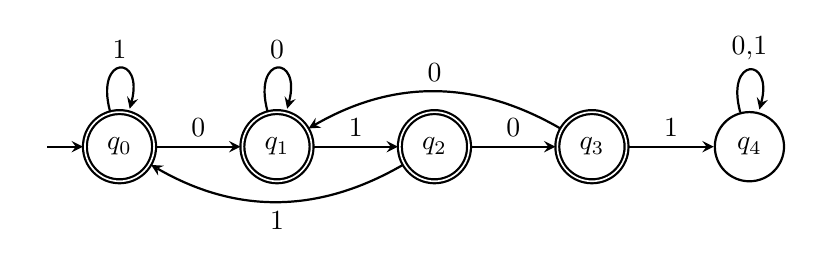
\begin{tikzpicture}[>=stealth,node distance=20mm,on grid,auto, thick, initial text=]
    \node[state,initial,accepting] (q0) {$q_0$};
    \node[state,accepting] (q1) [right=of q0] {$q_1$};
    \node[state,accepting] (q2) [right=of q1] {$q_2$};
    \node[state,accepting] (q3) [right=of q2] {$q_3$};
    \node[state] (q4) [right=of q3] {$q_4$};
    
    \path[->]
    (q0) edge [loop above] node {1} (q0)
    (q0) edge node {0} (q1)
    (q1) edge node {1} (q2)
    (q1) edge [loop above] node {0} (q1)
    (q2) edge node {0} (q3)
    (q2) edge [bend left] node {1} (q0)
    (q3) edge [bend right] node [above] {0} (q1)
    (q3) edge node {1} (q4)
    (q4) edge [loop above] node {0,1} (q4);    
  \end{tikzpicture}

\end{document}